%%%%%%%%%%%%%%%%%%%%%%%%%%%%%%%%%%%%%%%%%%%%%%%%%%%%%%%%%%%%%%%%%%%%%%%%%%%%%%%%
% Copyright 2021 Louis Paternault --- http://ababsurdo.fr
%
% Publié sous licence Creative Commons Attribution-ShareAlike 4.0 International (CC BY-SA 4.0)
% http://creativecommons.org/licenses/by-sa/4.0/deed.fr
%%%%%%%%%%%%%%%%%%%%%%%%%%%%%%%%%%%%%%%%%%%%%%%%%%%%%%%%%%%%%%%%%%%%%%%%%%%%%%%%

% Compiler avec lualatex:
%$ lualatex $basename

\documentclass[12pt, tikz]{standalone}

\usetikzlibrary{calc}

\begin{document}

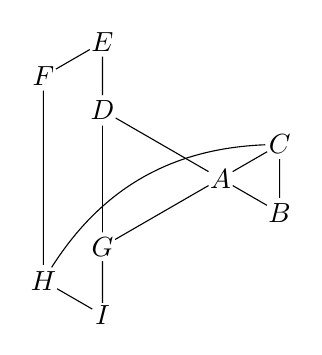
\begin{tikzpicture}
  \tikzstyle{sommet}=[circle, fill=white, minimum size=0em, inner sep=0];

  \coordinate (A) at (0:1);
  \coordinate (D) at (120:1);
  \coordinate (G) at (240:1);
  \begin{scope}[shift={($1.5*(A)$)}]
    \coordinate (B) at (-60:.5);
    \coordinate (C) at (60:.5);
  \end{scope}
  \begin{scope}[shift={($1.5*(D)$)}]
    \coordinate (E) at (60:.5);
    \coordinate (F) at (180:.5);
  \end{scope}
  \begin{scope}[shift={($1.5*(G)$)}]
    \coordinate (H) at (180:.5);
    \coordinate (I) at (300:.5);
  \end{scope}

  \draw (A) -- (B) -- (C) -- (A) -- (D) -- (E) -- (F) -- (H) -- (I) -- (G) -- cycle;
  \draw (D) -- (G);
  \draw (F) -- (H);
  \draw (H) to[bend left] (C);
  \draw (A) node[sommet]{$A$};
  \draw (B) node[sommet]{$B$};
  \draw (C) node[sommet]{$C$};
  \draw (D) node[sommet]{$D$};
  \draw (E) node[sommet]{$E$};
  \draw (F) node[sommet]{$F$};
  \draw (G) node[sommet]{$G$};
  \draw (H) node[sommet]{$H$};
  \draw (I) node[sommet]{$I$};
\end{tikzpicture}

\end{document}
